\section{Evaluation and Results}
\label{sec:evaluation-and-results}

We seek to evaluate whether \textsc{Appjudicator} is able to successfully
achieve its goal of distinguishing user-initiated network flows using UI
context, and whether it can do so with acceptable overhead. To determine whether
the app accomplishes its goal we perform a practical analysis and to measure the
app's resource cost we perform a performance evaluation. We now explain the
procedures used for each of these experiments and their results.

\subsection{Differentiating User-generated Flows}
\label{sec:differentiating-user-generated-flows}

The goal of this experiment is to determine whether \textsc{Appjudicator} can
successfully distinguish between network flows that were specifically initiated
by a human user and flows generated automatically by an app or the Android
system. We attempt to justify the parameters used for defining a flow as ``user
initiated.''

\subsubsection{Experimental Setup}
\label{sec:experimental-setup}

This test was performed on a virtual Google Pixel 4, with API level 30 (the
newest available). We perform actions on the phone to simulate real life use
cases with \textsc{Appjudicator}, including browsing the web in Chrome,
exploring an app store (F-Droid), and playing a game with advertisements. We use
our app's logging to record whether each flow is considered ``user initiated,''
along with the timing of UI interactions and flow table lookups.

To evaluate the effectiveness of our UI element system for identifying UI
elements (described in Section~\ref{sec:identifying-ui-elements}), we record
the proportion of accessibility events in our sampling period came from sources
with a unique resource ID.

\subsubsection{Results}
\label{sec:practical-results}

\textsc{Appjudicator} was successful in identifying 100\% of new flows that
occurred within two seconds of a UI interaction as user initiated. This raises
the question of how effective this two second cutoff is. Based on our
experience, two seconds seems to be generous enough to allow all flows
associated with the UI interaction to be triggered, without being so lenient
that unrelated flows are also allowed.

Professional sources generally support this reasoning. Google's developer blog
recommends two seconds of total page page load time is ``the threshold for
ecommerce site `acceptability.'"~\cite{ohye2010} Search engine optimization firm
Semrush writes ``Serve your customers with the page load time they need, a good
goal being 1--2 seconds.''~\cite{bird2020}

Figure~\ref{fig:lookups-after-click} shows illustrates this cutoff. It shows
four typical page loads in Chrome, with each point in the plot representing a
new flow made by Chrome. The accessibility event that initiated the page load
(clicking on a link) occurs at time 0. The dashed gray line shows the two second
cutoff. All the flows that occurred before this cutoff, within the green shaded
area, are considered to be user initiated, while flows that occurred after the
cutoff are not. These flows are likely the result of asynchronous JavaScript
network calls initiated by the page, not directly by user action.

\begin{figure}[h]
    \centering
	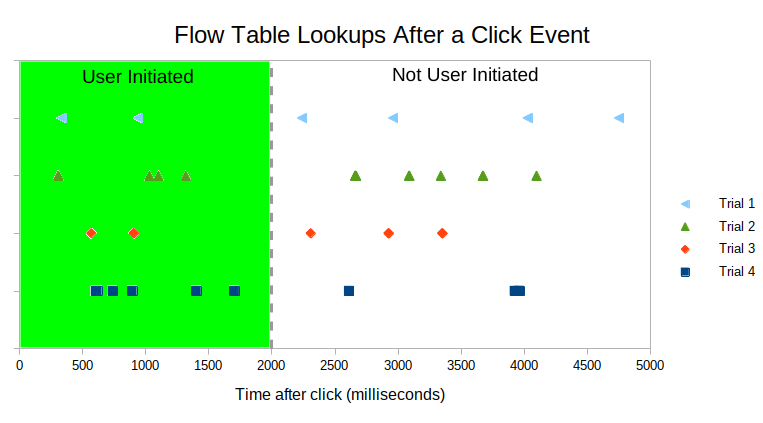
\includegraphics[width=\textwidth]{lookups-after-click.png}
	\caption{The delay between a click event and the new flows that it
		initiates. The dashed vertical line shows the two second cutoff: flows
		before this line (in the green area) are considered to be associated
		with the click event.}
	\label{fig:lookups-after-click}
\end{figure}

In our trial we found that approximately 85\% of accessibility events had a
source element with a unique resource ID. Even dynamically generated UI elements
often have resource IDs. For example, links in webpages are given IDs generated
by Chrome. This is good news for our system, because resource IDs are the
easiest and most effective way to uniquely identify UI elements form
accessibility events. Still, this figure may vary in poorly made apps in which
developers do not give every element an ID.

\subsection{Performance Evaluation}
\label{sec:performance-evaluation}

To fulfill its purpose as an always-enabled enterprise network security tool,
\textsc{Appjudicator} has to be as unobtrusive to end users as possible. This is
especially important because the app performs some actions on every network
flow, so any latency added by it would be especially noticeable.

\subsubsection{Measuring Added Latency}
\label{sec:measuring-added-latency}

To measure the effect of \textsc{Appjudicator} on network communication speed,
we measure the total additional latency added by the app. We measure added
latency in all incoming and outgoing packets, but focus on the first packet of
new TCP connections in particular, because these require the most processing
time.

For this test, we run the app in an Android virtual machine simulating a Google
Pixel 4, on API level 30. We use POX's \texttt{forwarding.hub} module as an
OpenFlow controller. In this mode, the controller responds to every query with
an instruction to forward the flow to its destination~\cite{mccauley2015}. Local
network latency is not a part of this test, so the controller server runs on the
same physical host as the Android virtual machine. The two components still
communicate over a regular TCP connection. The SDN agent starts with an empty
table of flow rules, so it must send a \texttt{packet\_in} to the controller for
every new flow. \textsc{Appjudicator} caches responses from the controller as
new rules, so subsequent connections to the same IP address and port over the
same protocol will not trigger a \texttt{packet\_in}.
Section~\ref{sec:openflow-protocol} describes the OpenFlow protocol in more
detail.

We focus particularly on the added latency of the first packet in a TCP
connection because this is where the system does the most processing. The start
of a new flow requires an SDN flow table lookup and possibly communication with
the SDN controller. Creating a new TCP connection requires allocating more
memory than a new UDP connection because metadata such as the current connection
state and most recent sequence number need to be stored in a lookup table.
Subsequent packets in a TCP flow, and all packets in UDP flows require less
processing overhead.

We configure the app to log a timestamp when a packet is first intercepted by
the VPN. \textsc{Appjudicator}'s VPN service parses the packet and determines
whether it is part of an existing connection or not, and adds it to a queue. If
it is the start of a new connection, the VPN service queries the SDN agent and
continues processing other packets while waiting for a response. The SDN agent
performs a flow table lookup, and sends a \texttt{packet\_in} to the SDN
controller if it fails to find a matching rule. If this is the case it waits for
a response from the controller, then performs a flow mod operation to cache the
result as a new rule. Finally the SDN agent instructs the VPN service to drop or
forward the flow. In this test all flows are allowed, so the VPN service removes
the packet from its queue and writes it to the correct network interface file
descriptor.\footnote{Figure~\ref{fig:packet-flow-chart} illustrates this
process.} Now that all of \textsc{Appjudicator}'s processing is finished a
second timestamp is logged. The earlier timestamp is the time the packet would
have been sent to the network without our system's interference, and the second
timestamp is the time it actually was sent. The difference is the total latency
added by the app.

In this test the app is configured to write the recorded time differences for
all packets to a file. Time differences for TCP SYN packets are also logged to
another file. Timestamps are created using Android's
\texttt{SystemClock.elapsedRealtimeNanos()} method, which gets the number of
nanoseconds since the system was booted.~\cite{androidsystemclock}

\subsubsection{Latency Test Results}
\label{sec:latency-test-results}

There were 1104 packet timing traces logged during the sampling period, of which
two were removed as outliers, leaving 1102 data points. The average added
latency among all packets was 5.14 milliseconds, with a standard deviation of
3.44 milliseconds.

During the sampling period 184 TCP SYN timing traces were logged, of which five
were removed as outliers, leaving 179 data points. These packets had 
higher added latency than others, and their added latency varied more. The
average added latency among TCP SYN packets was 14.64 milliseconds, with a
standard deviation of 16.77 milliseconds.

In our sample, 95\% of packets were processed with less than 10 milliseconds
of total added delay. On a 60 Hz display one frame lasts 16 milliseconds, so any
delay less than this is imperceptible to users.
Figure~\ref{fig:added-delay-chart} charts the full results of this test.

In measuring the timing of individual functions we found that the initial VPN
overhead (reading, processing, and queuing packets) took an average of 44
microseconds. Looking up flows in the flow table took an average of 53
microseconds with 10 initial rules, although this will increase as more flow
table entries are added. Accessibility event lookup took an average of 63
microseconds. By far the biggest contributor to overall latency in our trial was
sending \texttt{packet\_in} messages and waiting for a response from the
controller. The SDN agent waited 2448 microseconds on average for a
\texttt{packet\_out} message.

\begin{figure}[h]
    \centering
	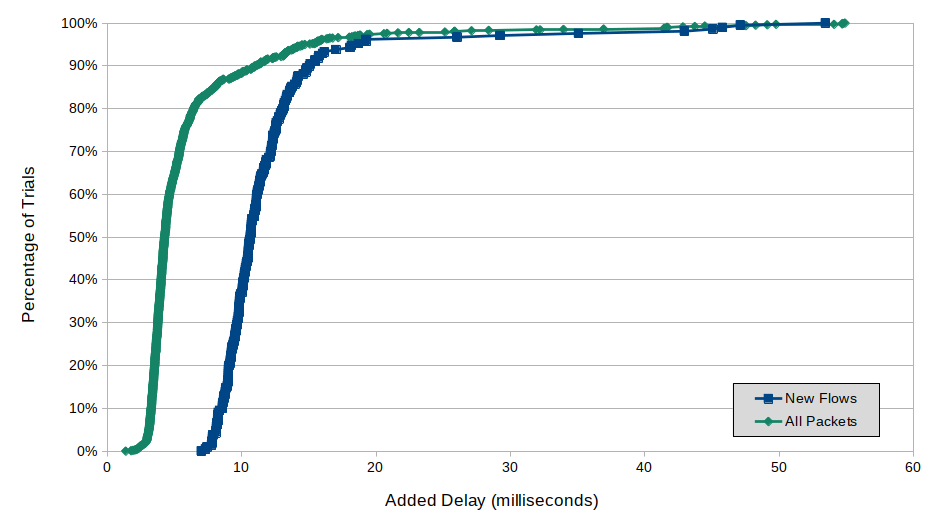
\includegraphics[width=\textwidth]{added-delay.png}
	\caption{Total latency added by \textsc{Appjudicator}}
	\label{fig:added-delay-chart}
\end{figure}

\subsubsection{Measuring Resource Overhead}
\label{sec:measuring-resource-overhead}

\textsc{Appjudicator} has costs in both added latency and increased resource
consumption. Running the VPN service, accessibility service, and SDN agent in
the background consumes additional processing cycles, memory, and battery life.
We measure the resource overhead with Android Studio's
Profiler.~\cite{androidprofiler}

This test was performed on an Android virtual machine simulating a Google Pixel
4, on API level 30. We ran the app the accessibility service, VPN service, and
SDN agent all enabled while recording its CPU, memory, and energy usage with
Android Studio's Profiler. The test lasted for 30 minutes, during which time we
used various other apps including Chrome, Termux, and F-Droid while
\textsc{Appjudicator} ran in the background.

During the trial, \textsc{Appjudicator}'s memory usage remained relatively
constant. It peaked at at 150.1 MB, with an average of 137.8 MB. Its processor
usage also usually remained low, averaging 5\% of the virtual machine's CPU but
occasionally spiking as high as 39\%. The profiler categorized the app's energy
usage as ``light,'' because it used only minor CPU resources and did not use any
location resources, wake locks, or alarms.

Based on these results, we conclude that \textsc{Appjudicator} has a minor
impact on CPU, memory, and battery usage on modern hardware, and therefore could
be used effectively as an always-on background security application.

\newpage

